
% Periodic boundaries conditions
% Germain Salvato-Vallverdu - may 2009
% http://germain.salvato-vallverdu.perso.sfr.fr
\documentclass[11pt,a4paper]{article}

\usepackage[utf8]{inputenc}
\usepackage{graphicx}

\usepackage{tikz}
\title{Periodic boundaries conditions}
\author{Germain Salvato-Vallverdu}

\usepackage{hyperref}
\hypersetup{%
pdfauthor={Morteza Jalambadani},%
pdftitle={Image-18},%
pdfkeywords={Tikz,latex,Image-18,Morteza Jalambadani},%
pdfcreator={PDFLaTeX},%
pdfproducer={PDFLaTeX},%
}

\newcommand\firstSquare{14cm}
\newcommand\secondSquare{10cm}
\newcommand\thirdSquare{6cm}
\newcommand\squareColor{black}
\newcommand\squareLineWidth{1.2mm}


\newcommand\circleColor{gray}
\newcommand\circleRadius{7pt}
\newcommand\circleLineWidth{0.9mm}


\newcommand\arrowColor{gray}
\newcommand\arrowLineWidth{1.5mm}

\newcommand\textSquareThird{Third Text}
\newcommand\textSquareSecond{Second Text}
\newcommand\textSquareFirst{First Text}



\pagestyle{empty}

\begin{document}

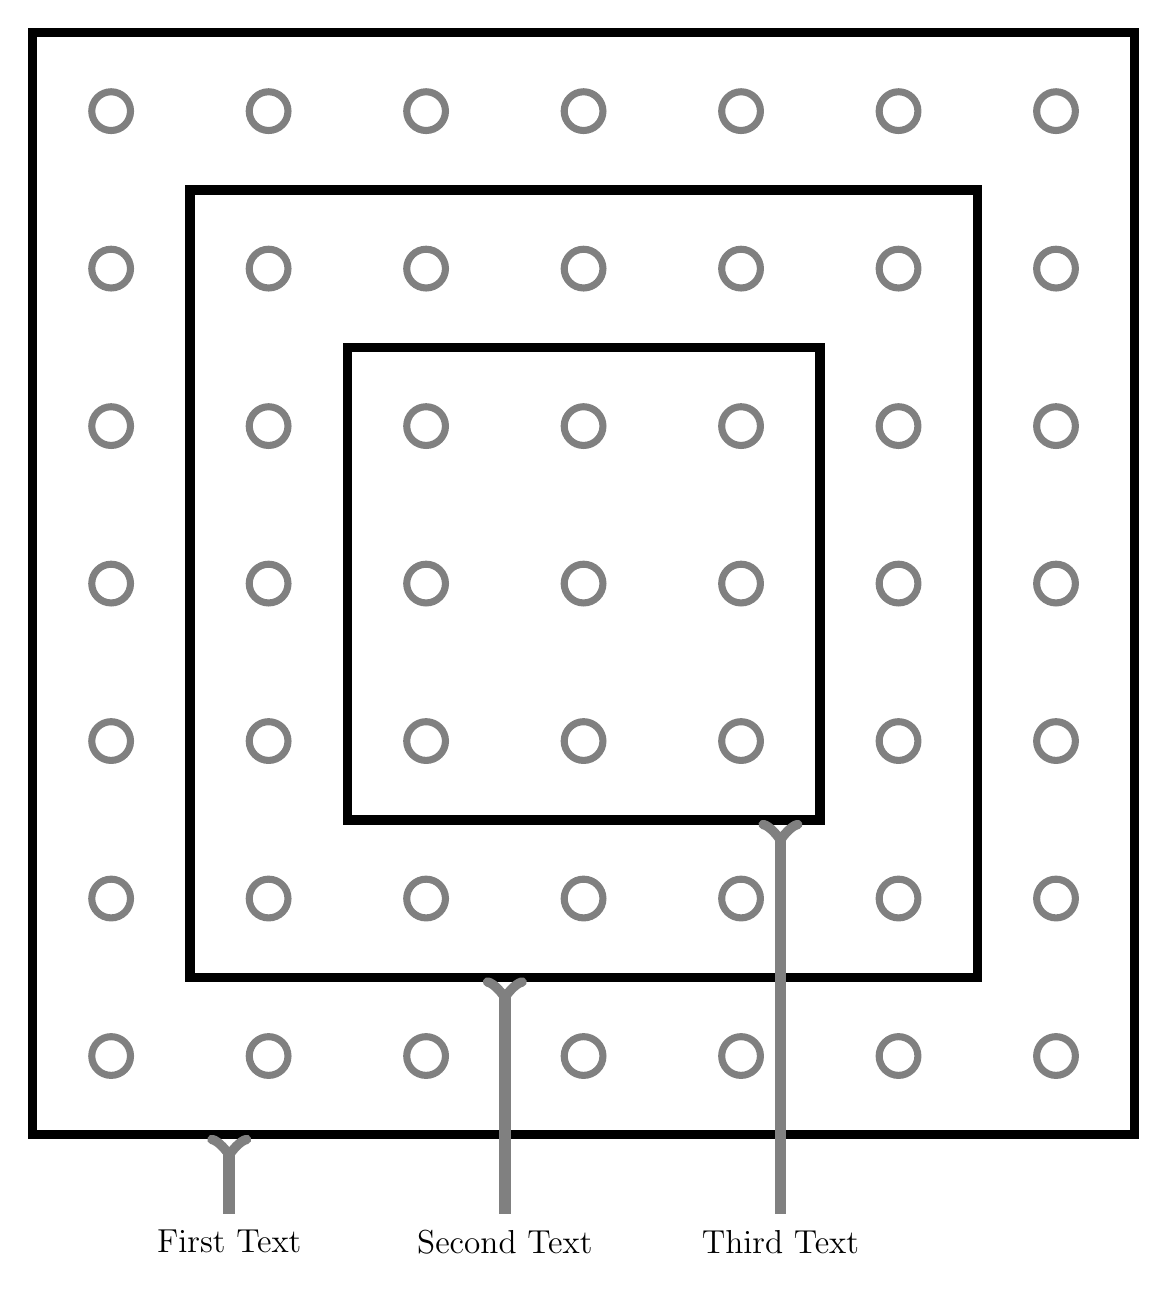
\begin{tikzpicture}


    \foreach \x in {-6,-4,...,6}{
        \foreach \y in {-6,-4,...,6}{
            \draw[line width=\circleLineWidth, \circleColor]  (\x,\y) {} circle (\circleRadius);
        }
    }
    % I want to center the rectangle here
    % drawing the node with shape=rectangle and anchor=center
    \node [draw=\squareColor,  thick, line width=\squareLineWidth, shape=rectangle, minimum width=\firstSquare, minimum height=\firstSquare, anchor=center] (Image18_Square_First) at (0,0) {};
    \node [draw=\squareColor,  thick, line width=\squareLineWidth, shape=rectangle, minimum width=\secondSquare, minimum height=\secondSquare, anchor=center] (Image18_Square_Second) at (0,0) {};
    \node [draw=\squareColor,  thick, line width=\squareLineWidth, shape=rectangle, minimum width=\thirdSquare, minimum height=\thirdSquare, anchor=center] (Image18_Square_Third) at (0,0) {};

    \draw [node font= \large, draw=\arrowColor,  thick, line width=\arrowLineWidth][>-]  (-4.5,-\firstSquare/2) --(-4.5,-8)  node[below] {\textSquareFirst};
    \draw [node font= \large, draw=\arrowColor,  thick, line width=\arrowLineWidth][>-]  (-1,-\secondSquare/2) -- (-1,-8)  node[below] {\textSquareSecond};
    \draw [node font= \large, draw=\arrowColor,  thick, line width=\arrowLineWidth][>-]  (2.5,-\thirdSquare/2) --(2.5,-8) node[below] {\textSquareThird};


\end{tikzpicture}


\end{document}

